% 2009 年江西卷理科第 21 题：双曲线 x^2/(8b^2)-y^2/b^2=1，右焦点 F2，P1 在双曲线上，
%   过 P1 作右准线的垂线，垂足 A，直线 F2A 交 y 轴于 P2，P 为 P1P2 的中点。
% 来源 PDF：gaokaomath-src/普通高考/2009/2009江西理.pdf
% SHA-256：64f70e9750ae2736476d825abdc20639c64a2dfe6c22493b64e710108d5c49e7
% 原页：2009江西理.pdf 第 2 页（A3 三栏）第 2 栏，书页码 534。
% 绘制依据：取 b=1，则 a=2√2≈2.83、c=3、右准线 x=8/3，顶点与焦点相距很近，
%   故把横向比例放大到 1cm/单位。取 P1 在左支上侧（y0=0.40，x0=-3.05），
%   A(8/3,0.40)，P2(0,3.60)，P 为 P1P2 中点；标签加白底并避开曲线。
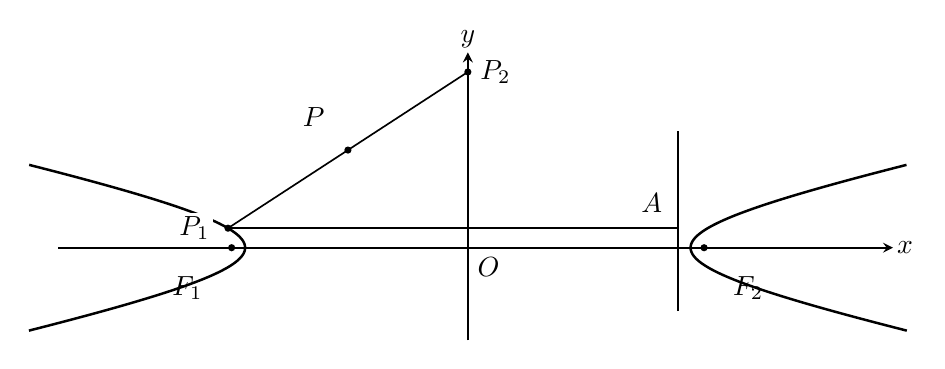
\begin{tikzpicture}[x=1.0cm, y=0.62cm, semithick, every node/.style={inner sep=1.2pt}]
  \draw[->,>=stealth] (-5.2,0) -- (5.4,0) node[right] {$x$};
  \draw[->,>=stealth] (0,-1.9) -- (0,4.0) node[above] {$y$};
  \node[below right=2pt] at (0,0) {$O$};

  % 双曲线两支
  \draw[line width=0.9pt, domain=-1.3:1.3, samples=90]
    plot ({2*sqrt(2)*cosh(\x)},{sinh(\x)});
  \draw[line width=0.9pt, domain=-1.3:1.3, samples=90]
    plot ({-2*sqrt(2)*cosh(\x)},{sinh(\x)});

  % 右准线
  \draw (2.6667,-1.3) -- (2.6667,2.4);

  \coordinate (P1) at (-3.046,0.40);
  \coordinate (A)  at (2.6667,0.40);
  \coordinate (P2) at (0,3.60);
  \coordinate (P)  at (-1.523,2.00);
  \coordinate (F1) at (-3,0);
  \coordinate (F2) at (3,0);

  % P1 到右准线的垂线、P1P2
  \draw (P1) -- (A);
  \draw (P1) -- (P2);

  \fill (P1) circle (1.3pt);
  \fill (P2) circle (1.3pt);
  \fill (P)  circle (1.3pt);
  \fill (F1) circle (1.3pt);
  \fill (F2) circle (1.3pt);

  \node[left=5pt, fill=white, inner sep=1.4pt] at (P1) {$P_1$};
  \node[above left=4pt, fill=white, inner sep=1.4pt] at (A) {$A$};
  \node[right=3pt] at (P2) {$P_2$};
  \node[above left=7pt] at (P) {$P$};
  \node[below left=9pt] at (F1) {$F_1$};
  \node[below right=9pt] at (F2) {$F_2$};
\end{tikzpicture}
